\chapter{Background}\label{ch:background}

\section{Nuclear Magnetic Resonance}

Nuclear Magnetic Resonance (NMR) is an effect most often associated with chemical spectroscopy, or magnetic resonance imaging.
This work in this thesis is closer to the technique of NMR relaxometry, the study of relaxation.
This section will give a brief overview of the physics of NMR, using the semi-classical model and the Bloch equations.
It describes NMR occuring to protons (\textsuperscript{1}H), which is the most common nucleus used for NMR and what is used in this thesis, although NMR can be observed with any nuclei with non-zero spin.
For a more complete discussion, the reader is directed to one of the many textbooks on the subject, including books by Abragham\cite{AbragamPrinciplesNuclearMagnetism1961} and Callaghan\cite{CallaghanPrinciplesNuclearMagnetic1994} or Brown et al.\cite{BrownMagneticResonanceImaging2014a}.

Protons have an magnetic moment due to their intrinsic angular momentum, or `spin'.
To observe nuclear magnetic resonance, protons are put into a magnetic field (\Bzero) that interacts with the protons magnetic moment, lowering the energy of magnetic moments aligned with \Bzero (along \textit{z}).
Following the Boltzman distribution, this energy difference causes an increase in the fraction of protons in the lower energy state, generating a net magnetisation aligned with the \Bzero field.
As the size of the net magnetisation depends on the relative difference of spins towards and against the field, the net magnetisation becomes stronger when a larger \Bzero field is used.
Any imbalance created is typically very small, which means that the NMR signal generated is very weak.

A magnetic moment in a magnetic field experiences a torque, which causes it to rotate around an axis along the magnetic field.
This is called Larmor precession, and gives rise to the Larmor frequency $\omega$, which defines the rate of rotation.
Protons in a magnetic field precess at a frequency given by \autoref{eq:back-larmor}, where $\gamma$ is the gyromagnetic ratio (\SI{2.56e8}{rads^{-1}T^{-1}} for protons).
At equilibrium, the net magnetisation is along \textit{z}, so precession is not visible.

\begin{equation}
\omega = \gamma B_0
\label{eq:back-larmor}
\end{equation}

The effect of the \Bone field can be seen by considering a frame (\textit{x', y', z'}) which rotates around the \textit{z} axis at this precession frequency (a `rotating frame', when compared to the stationary `lab frame')
In the rotating frame, the net magnetisation still lies along the \textit{z}-axis.
Applying an additional magnetic field, along \textit{x'} (i.e. perpendicular to \Bzero) to the \textit{z}-axis causes the magnetisation to rotate around \textit{x'} towards \textit{y'}, following the same precession principle.
The strength and time that the \Bone field is applied for can be changed to control the amount of rotation, leading to \SI{90}{\degree} and \SI{180}{\degree} pulses.

\begin{figure}[t]
\centering
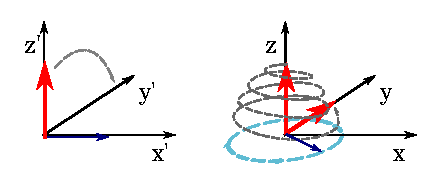
\includegraphics[width=0.7\textwidth]{figures/background/fid.pdf}
\caption[Effect of the \Bone field]{Applying a \Bone field along \textit{x'} causes the magnetisation to rotate towards \textit{y'}. Transforming this to the laboratory frame shows that the \Bone field must oscillate at the precession rate, and causes the magnetisation to spiral down into the transverse (\textit{xy}) plane}
\label{fig:back-fid}
\end{figure}

Transforming this into the lab frame means that the \Bone field becomes a magnetic field oscillating at the Larmor frequency,
while the components of the magnetisation along \textit{x} and \textit{y} correspond to a rotating magnetisation in the sample.
This produces the resonance condition for NMR -- the frequency of the \Bone field needs to match the precession frequency to cause maximum rotation.
These can be created and detected using a coil, as the rotating magnetic field from the sample induces a voltage in the coil due to Faraday's Law.
This NMR signal is known as the Free Induction Decay (FID).

\section{\Tone and \Ttwo relaxation}
The NMR signal from a sample decays due to relaxation with two main mechanisms.
It can be caused by the return of net magnetisation to equilibrium, or by a loss of coherence across a sample.

As mentioned above, the equilibrium state of a sample in a \Bzero field is for the net magnetisation to align with the \Bzero magnetic field.
When this is disturbed, for example, in an NMR experiment or when the sample is first placed in the \Bzero field, the protons in the sample exchange energy to return to the equilibrium.
This process, also known as spin-lattice relaxation, is described by \autoref{eq:back-Tone}, where M\textsubscript{0} is the equilibrium magnetisation, and the time constant for relaxation is \Tone.

\begin{equation}
\frac{\mathrm{d} M_z}{\mathrm{d} t} = \frac{1}{T_1} (M_0-M_z)
\label{eq:back-Tone}
\end{equation}

The \Tone of a sample can be determined by an inversion recovery experiment.
A \SI{180}{\degree} pulse is applied to the sample, and the magnetisation remaining is measured after a range of variable delay time ($t_d$ )by applying a \SI{90}{\degree} pulse and taking the intensity of the FID.
This can be used to fit a curve with the equation
\begin{displaymath}
M(t_d) = M_0 (1 - 2 e^{-\frac{t_d}{T_1}})
\end{displaymath}

\begin{figure}[t]
\centering
\makebox[\textwidth][c]{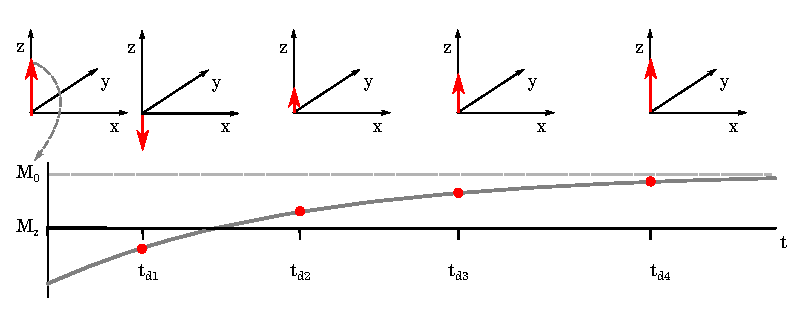
\includegraphics[width=1.1\textwidth]{figures/background/T1relaxation.pdf}}
\caption[Inversion recovery experiment]{\Tone relaxation leads to the recovery in the equilibrium magnetisation (M\textsubscript{0}). The Inversion Recovery experiment works by applying a \SI{180}{\degree} pulse, then measuring the magnetisation by applying a \SI{90}{\degree} pulse at time \textit{t\textsubscript{d}} to generate an FID. Repeating the experiment with a range of \textit{t\textsubscript{d}}s allows the samples \Tone to be measured.}
\label{fig:back-T1}
\end{figure}

In most cases, the \Tone controls how rapidly an experiment can be repeated.
A general rule is to set the repetition time (\TR - the delay between experiments) to 5$\times$\Tone, so that the sample magnetisation recovers to \SI{>99}{\percent} of its original equilibrium level.
Otherwise the signal produced will be weaker, as it depends on the magnetisation along the \textit{z} axis.
This also removes any remaining transverse magnetisation, as the protons return to equilibrium.
Because of this, \Ttwo < \Tone.

The \textit{x} and \textit{y} components of a sample's magnetisation (the transverse magnetisation) also undergoes relaxation.
The transverse magnetisation is generated by the combination of magnetisation from protons across the sample.
The NMR signal is generated when the magnetic moments of all of the protons in a sample precess at the same rate, and are all aligned in the same direction (i.e. have the same phase), creating coherence.
If protons in part of the sample experience a different magnetic field, they precess at a different rate and lose coherence with the rest of the sample.
This reduces the overall transverse magnetisation of the sample, which decreases following \autoref{eq:back-Ttwo}, where \Ttwo is the time constant for this relaxation.

\begin{equation}
\frac{\mathrm{d}M_{xy}}{\mathrm{d}t} = - \frac{1}{T_2} (M_{xy})
\label{eq:back-Ttwo}
\end{equation}

\begin{figure}[t]
\centering
\makebox[\textwidth][c]{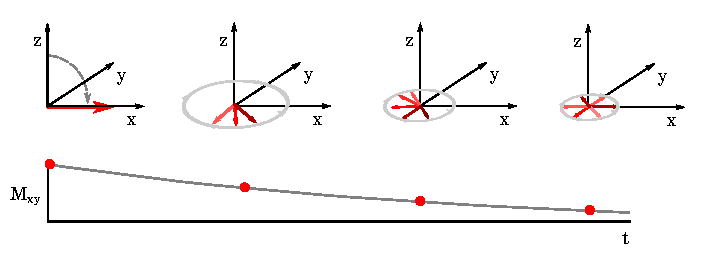
\includegraphics[width=1.1\textwidth]{figures/background/T2relaxation.pdf}}
\caption[Transverse relaxation due to an inhomogeneous field]{Variations in the \Bzero field cause protons in different locations to precess at different rates (shown in red shading). As the total magnetisation is the sum of the proton magnetic moments, the different magnetisations start cancelling out and cause a decay in the transverse component of the magnetisation, called \Ttwostar relaxation.}
\label{fig:back-T2}
\end{figure}

In a physical sample, protons are always experiencing different magnetic fields due to the fluctuating magnetic moments of surrounding protons.
The dephasing from this process is random and non-reversible.
The physical properties of a sample control the amount of interaction between protons on surrounding molecules, and the rates of this intrinsic \Ttwo relaxation, for example, solids have extremely fast \Ttwo relaxation times, on the order of 10s of microseconds, while water can have a \Ttwo on the order of seconds.

\Ttwo relaxation can also be increased by the presence of paramagnetic ions in the sample, such as Cu\textsuperscript{2+}, Mn\textsuperscript{2+} and Gd\textsuperscript{3+}.
These affect the magnetic fields experienced by protons in the sample, and cause additional dephasing.
Their effect is characterised by a relaxivity \textit{r}, measured in \si{s^{-1}/mmolL^{-1}}, which describes the dependence on concentration.
This is due to the additive nature of relaxation rates: when multiple processes cause relaxation, the relaxation rates add together

\begin{displaymath}
\frac{1}{\Ttwo} = R_2 = \frac{1}{T_{2 intrinsic}} + r_{2} c_{metal}
\end{displaymath}

Additionally, another process reduces the transverse magnetisation of a sample.
\Ttwostar relaxation is associated with the homogeneity of the \Bzero field, as different magnetic fields across the sample will produce different precession rates, and cause protons to dephase.
This process is illustrated in \autoref{fig:back-T2}.

The precession of the net magnetisation around the \Bzero field, and the effect of relaxation on the net magnetisation can be expressed using the phenomelogical Bloch equation \autoref{eq:back-Bloch}.

\begin{equation}
\frac{\mathrm{d}\mathbf{M}}{\mathrm{d}t} = \gamma \mathbf{M} \times \mathbf{B} + \frac{1}{T_1} (M_0 - M_z) - \frac{1}{T_2} M_{xy}
\label{eq:back-Bloch}
\end{equation}

\section{Spin echoes and CPMG}
\label{sec:back-spinecho}
The spin echo was first described by Hahn in 1950\cite{HahnSpinEchoes1950}.
By applying a \SI{180}{\degree} pulse a time $\tau$ after a \SI{90}{\degree} pulse, he observed a signal forming at $2\tau$.
He showed that this is due to the spread of phase caused by the \Bzero field inhomogeneity being reversed, which allows the protons to rephase and regenerate a net transverse magnetisation that can be detected.

\begin{figure}[t]
\centering
\makebox[\textwidth][c]{
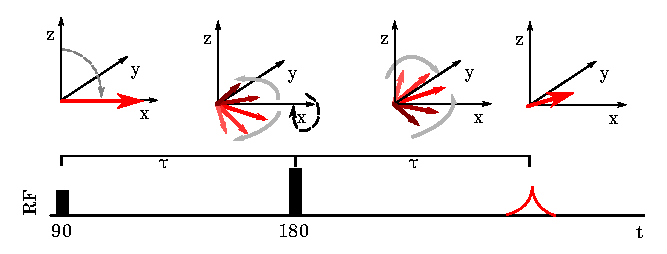
\includegraphics[width=1.1\textwidth]{figures/background/Spinecho.pdf}}
\caption[Generation of a Spin echo]{Generation of a spin echo: as protons precess at different rates, they accumulate different amounts of phase (shown by red shading). Applying a \SI{180}{\degree} pulse a time $\tau$ after the \SI{90}{\degree} pulse causes the magnetisation to be rotated around the \textit{x}-axis, so the different rates unwind their different phases, producing an echo at $2\tau$.}
\label{fig:back-spinecho}
\end{figure}

The formation of the spin echo is shown illustrated in \autoref{fig:back-spinecho}.
The inhomogeneous \Bzero field causes protons across the sample to have different Larmor frequencies, meaning that they precess at different rates, and accumulate different amounts of phase as time continues.
The different phases cause the net transverse magnetisation of the whole sample to decay, with a shorter time constant \Ttwostar.
Applying a \SI{180}{\degree} refocusing pulse $\tau$ after the \SI{90}{\degree} pulse causes the magnetic moments of each proton to rotate through \SI{180}{\degree} around the \textit{x} (or \textit{y}) axis, so that the different precession rates unwind the different accumulated phase.
Thus unwinding causes the magnitude of the net transverse magnetisation to increase, reaching a maximum at $2\tau$, which is the centre of the echo.
The spin echo will still have a reduced intensity, due to the intrinsic \Ttwo relaxation proceses described above.
However, it removes the effects of the inhomogeneous \Bzero field, and allows the measurement of the intrinsic \Ttwo relaxation process.

This rephasing process relies on the protons experiencing the same \Bzero field in the period before and after the \SI{180}{\degree} pulse.
If protons move across an inhomogeneous field during this time, they may not experience the same field and not be complete refocussed at $2\tau$.
This can be due to diffusion (the random movement of protons in the sample) or processes such as chemical exchange (explored below).

\begin{figure}[t]
\centering
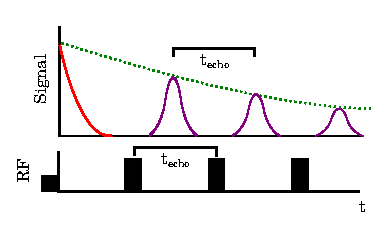
\includegraphics[width=0.7\textwidth]{figures/background/cpmg.pdf}
\caption[CPMG pulse sequence]{Repeatedly applying \SI{180}{\degree} pulses produces a series of spin echoes. Measuring the intensity of the echoes (purple) allows the true \Ttwo relaxation (green) to be measured.}
\label{fig:back-cpmg}
\end{figure}

Once the magnetisation has been refocused in the spin echo, the transverse magnetisation decays following the \Ttwostar relaxation time again.
Carr and Purcell proposed repeating the refocussing pulses, to create more echoes and further map out the \Ttwo relaxation \cite{CarrEffectsDiffusionFree1954}.
In this experiment, the refocussing pulses are evenly spaced by an echo time, as shown in \autoref{fig:back-cpmg}.
Meiboom and Gill improved this experiment by adjusting the phase of the \SI{180}{\degree} pulses relative to the \SI{90}{\degree} pulse, such that they rotate the magnetisation around the \textit{y}-axis rather than \textit{x}-axis \cite{MeiboomModifiedSpinEcho1958}.
This reduces the errors caused by an incorrect \SI{180}{\degree} pulse.
With this modification, the CPMG experiment is commonly used for fast and robust measurements of the \Ttwo of a sample.

\begin{equation}
S(t) = S_0 e^{\frac{t}{T_2}}
\label{eq:CPMGT2fitting}
\end{equation}
The intensity of echoes in a CPMG experiment follows a monoexponential decay (for samples with a single relaxation component).
The \Ttwo can be measured by the slope of a semi-log plot, or by non-linear fitting of the function \ref{eq:CPMGT2fitting}.
While measurements of the intrinsic \Ttwo should not be afffected by the echo time used, process like exchange and diffusion can alter the measured \Ttwo.
For example, for protons moving in a magnetic gradient, a longer echo time means that protons experience a wider range of \Bzero fields before being refocussed.
This makes the refocusing less effective, and results in a shorter observed \Ttwo, following \autoref{eq:CPMGgrad}.
Similarly, exchange processes can cause protons to experience different magnetic fields in the timescale of the experiment, causing the refocusing to be less efficient.
Exchange processes, and their applicability to blood are discussed further in \autoref{sec:back-T2SO2}.

\begin{equation}
\frac{1}{T_2} = \frac{1}{T_2} + \frac{\gamma^2 G^2 D \tau^2}{12}
\label{eq:CPMGgrad}
\end{equation}

\section{PGSE experiments}
\label{sec:back-PGSE}
Pulsed Gradient Spin Echo (PGSE) experiments combine the spin echo with magnetic field gradients to measure the displacement of protons in a sample.
Traditionally, a magnetic field gradient creates a known change in the \Bzero field, which is linearly related to its position: $B_0(z) = B_0 + g(z)$
This allows protons to be spatially resolved, as they will have different Larmor precession frequencies at different locations.
This principle is the basis of Magnetic Resonance Imaging (MRI).

\begin{figure}[t]
\centering
\makebox[\textwidth][c]{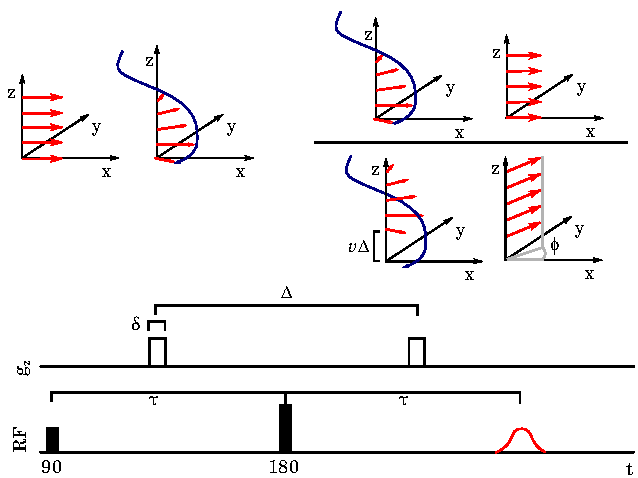
\includegraphics[width=0.8\textwidth]{figures/background/pgse.pdf}}
\caption[Pulsed Gradient Spin Echo (PGSE) experiment]{Pulsed Gradient Spin Echo experiment: Applying a gradient changes the precession frequency to be dependent on the position along z, and imparts a phase difference depending on the time it is active($\delta$) (shown by the blue helix). Using a spin echo, and repeating the gradient pulse will unwind the this added phase if the protons have not moved (upper image). If the protons have moved together (e.g. flow), the second gradient pulse will bring them back into phase with each other, but leave an additional phase ($\phi$) which can be measured to determine the displacement.}
\label{fig:back-pgse}
\end{figure}

Stejskal and Tanner proposed the PGSE experiment in 1965 \cite{StejskalSpinDiffusionMeasurements1965}.
Their experiment uses a pulsed magnetic field gradient, which creates a range of precession rates across the sample for a short time, so that protons accumulate a phase related to their position.
A \SI{180}{\degree} pulse is then applied, and an identical pulsed field gradient is reapplied.
This causes the phase accumulated in the first pulse to be reversed before the spin echo is formed.
Assuming there is no movement, the protons in the sample will be completely rephased, and the normal spin echo will be recovered.

Diffusion (random movement) of protons means that the rephasing is not as effective, as the phase accumulated in the first pulsed gradient will not be totally removed.
This means that some of the protons will cancel each other out, and cause the intensity of the spin echo to be reduced.
By running experiments with a range of gradient strengths (\textit{g}) and measuring the echo intensity, the diffusion coefficient (D) for the sample can be obtained using \autoref{eq:PGSEdiff}, where $\delta$ is the length of time the pulsed gradient field is active, and $\Delta$ is the time between the two gradient pulses.

\begin{equation}
S(G) = S_0 e^{-\gamma^2 G^2 \delta^2 (\Delta - \frac{\delta}{3} ) D}
\label{eq:PGSEdiff}
\end{equation}

In contrast, uniform motion of protons in a sample (such as flow) produces a different effect.
Rather than the intensity of the spin echo decreasing, the phase of the spin echo is shifted.
That is, the spin echo will form with the transverse magnetisation rotated slightly around the \textit{xy} plane when compared to a measurement with no flow (or no gradient), as the second gradient pulse `overcorrects' the dephasing.
The velocity of the sample can be determined using two methods \cite{CallaghanVelocitydiffusionimaging1991,XiaOneshotvelocitymicroscopy1992,CallaghanTranslationalDynamicsMagnetic2014}
By measuring the phase and intensity at a range of gradient strengths, the velocity can by found using a Fourier transform.
This produces a spectrum with a peak at the propagator, the average displacement in the sample.
Alternatively, taking the phase ($\phi$) of the echo measured with a single gradient strength, and comparing it to a reference where there is no gradient, the flow velocity can be measured using \autoref{eq:PGSEvel}.
This second `one-shot' method was used in these experiments, as it requires less measurements than the Fourier method to complete the same measurement.
\begin{equation}
v = \frac{\phi}{\gamma \Delta \delta g}
\label{eq:PGSEvel}
\end{equation}

\section{Blood and oxygen saturation}

Blood contains multiple components, including red blood cells, white blood cells, platelets, and plasma.
Red Blood Cells (RBCs) are associated with oxygen tranport, while white blood cells are part of the immune system.
Platelets are involved in the blood clotting process, and plasma is the mixture of water, nutrients and proteins which these components are suspended in.
Blood is pumped around the circulatory system by the heart, and transports nutrients to all parts of the body.
On average, blood makes up 7\% of a person's body weight, making a volume of about \SI{5}{L}.

In addition to the nutrients carried in the plasma,  blood is responsible for the tranport of oxygen from the lungs to the body.
Most of the oxygen transported is carried by red blood cells, with a small amount dissolved in blood plasma (typically \SI{<3}{\percent}).
These are shown in \autoref{fig:back-bloodcell}, and have a biconcave disc shape, with a mean diameter of \SI{7.8}{\micro\metre}, and mean thickness of \SI{2.5}{\micro\metre}.
RBCs contain no cell nucleus and are very deformable, which allows them to travel through narrow capillaries in tissue.
While they have no nucleus, they still metabolise slowly to maintain membrane deformability and ion transport through the cell membrane.
RBCs have a typical lifetime in the body of 120 days.

The fraction of blood volume in red blood cells is called the haematocrit (typically around 0.4 in healthy adults)
The primary role of RBCs is to contain and transport haemoglobin in the blood, and they can contain very high concentrations (up to \SI{34}{g/L}) of haemoglobin inside.

\begin{figure}[t]
\centering
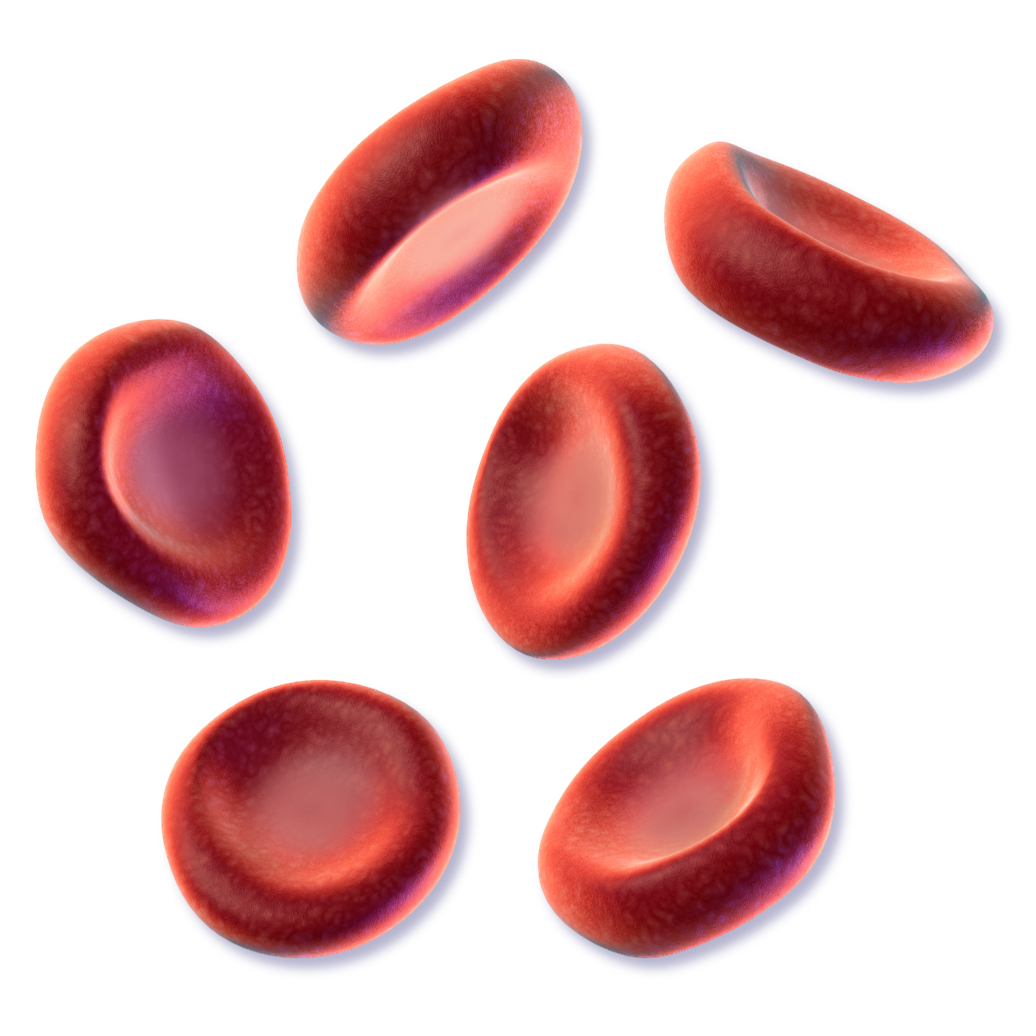
\includegraphics[width=0.5\textwidth]{figures/background/Blausen_0761_RedBloodCells_crop.png}
\caption[Illustration of red blood cells]{Illustration of red blood cells. Source: Bruce Blaus \url{https://commons.wikimedia.org/wiki/File:Blausen_0761_RedBloodCells.png}}
\label{fig:back-bloodcell}
\end{figure}

\section{Oxy- and deoxy-haemoglobin}
\label{sec:back-po2so2}
Haemoglobin is a protein which can reversibly bind to oxygen to improve  its transport in the body. \cite{HallGuytonHallTextbook2015}
By binding the oxygen to haemoglobin, blood can transport 30-100 times more oxygen than relying on dissolved oxygen in the plasma.
It contains four heme groups, each containing an iron ion (Fe\textsuperscript{2+}) which can reversibly bind to oxygen.
In the lungs, oxygen diffuses into the blood and RBCs, and is taken up by haemoglobin to form oxy-haemoglobin.
This increases the oxygen saturation (\SOtwo), which is defined as the fraction of all haemoglobin bound to oxygen in \autoref{eq:o2sat} (in terms of concentration)\cite{ToffalettiMisconceptionsreportingoxygen2007}.

\begin{equation}
sO_2 = \frac{c_{oxyHb}}{c_{oxyHb} + c_{deoxyHb}}
\label{eq:o2sat}
\end{equation}

After leaving the lungs, the \SOtwo will be around 97\%, and the p\Otwo (the partial pressure of oxygen - proportional to the concentration of \Otwo) will be around \SI{95}{mmHg}.
As blood travels around the body, oxygen diffuses from the blood into the tissue, which has a lower p\Otwo due to metabolism.
The oxygen dissolved in plasma decreases, decreasing the p\Otwo.
This change triggers the oxy-haemoglobin to release oxygen, forming deoxy-haemoglobin and effectively buffering the p\Otwo change.
In venous blood, after leaving tissue, the \SOtwo will be between \SIrange{20}{70}{\percent}, and have a p\Otwo between \SIrange{20}{40}{mmHg} (depending on the demand for oxygen in the tissue). \cite{HallGuytonHallTextbook2015}

In addition to these two forms of haemoglobin, other dys-haemoglobins can also be created, including met- and carboxy-.
Met-haemoglobin is formed when the iron in the complex is further oxidised to Fe\textsuperscript{3+}.
Carboxy-haemoglobin is formed when carbon monoxide (CO) binds to haemoglobin, forming a bond much stronger than oxygen does, and leading to the loss of oxygen transport capacity.
These other forms are not expected to be created in this experiment.

\begin{figure}[t]
\centering
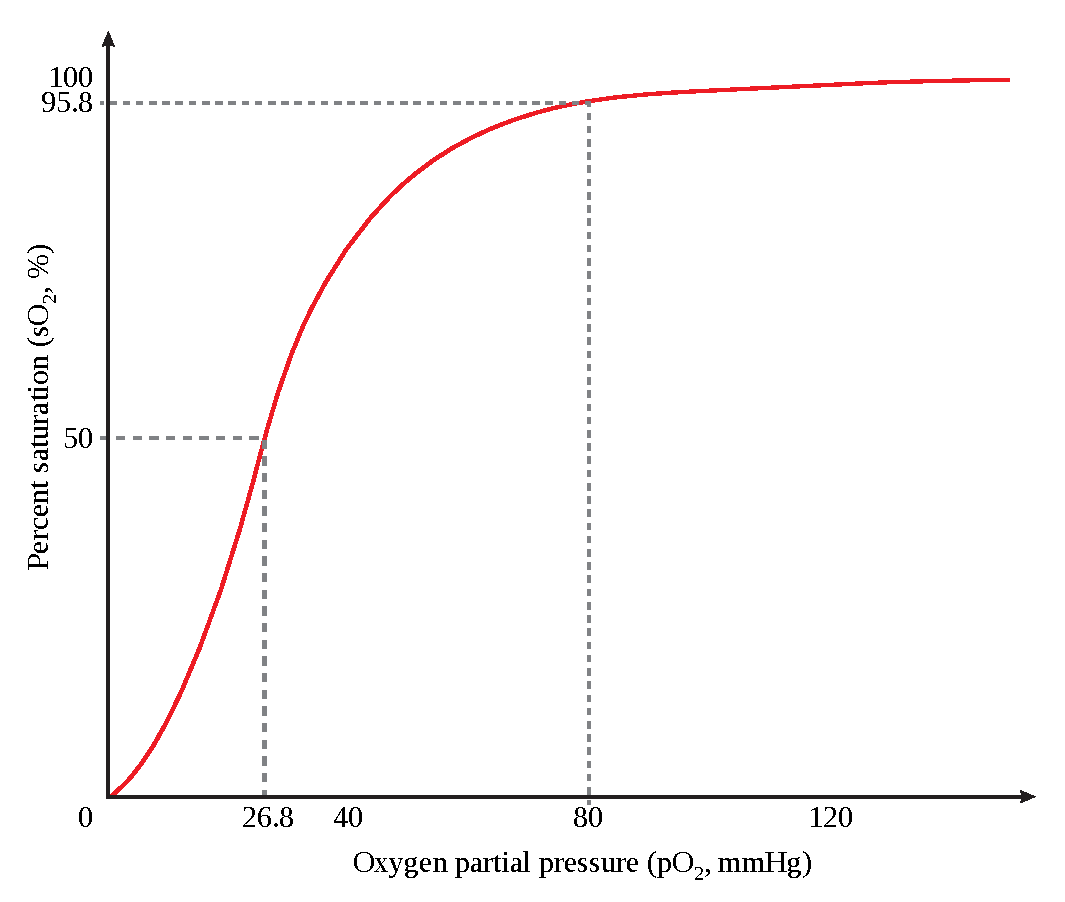
\includegraphics[width=0.7\textwidth]{figures/background/Hemoglobin_saturation_curve.pdf}
\caption[Graph showing relationship between p\Otwo and \SOtwo in blood]{Graph showing relationship between p\Otwo and \SOtwo in human blood. Source: \url{https://commons.wikimedia.org/wiki/File:Hemoglobin_saturation_curve.svg}}
\label{fig:back-po2so2}
\end{figure}

The relationship between \SOtwo and p\Otwo is non-linear due to effects such as co-operative binding.
Binding the first oxygen molecule to one of the heme groups causes a change in the shape of the protein which makes binding at the other heme groups easier.
This makes the \SOtwo increase more steeply (as a function of p\Otwo) once the first oxygen is bound.
This effect also works in reverse, causing the protein to release oxygen.
Physiologically, this causes a release of oxygen in areas with low p\Otwo, which helps to deliver oxygen to tissue that needs it.

Other factors also affect the relationship between \SOtwo and p\Otwo. \cite{HallGuytonHallTextbook2015}
One example is the pH, where an increase in acidity (e.g. 7.4 to 7.2) causes an decrease in oxygen affinity, and the release of more oxygen from haemoglobin.
This dependency underlies the Bohr effect:
pH in the blood is also affected by dissolved \COtwo, which exists in equilibrium with carbonic acid in the blood.
An increased p\COtwo causes more carbonic acid to be formed, lowering the pH of the blood.
This causes oxygen to be released in areas where \COtwo is being produced due to metabolism.

Changes in the \SOtwo can be measured using the different optical and magnetic properties of oxy- and deoxy-haemoglobin.
The binding of oxygen to haemoglobin causes them to have slightly different optical absorption spectra.
In particular, the deoxy-haemoglobin absorbs strongly in the red region of the spectrum.
This causes a colour change, where oxygenated blood appears red, and deoxygenated blood appears almost black.

Oxygen binding to haemoglobin also causes a change in the electronic structure of the iron atom. \cite{PaulingMagneticPropertiesStructure1936}
In the oxygenated state, the iron atom complex has no unpaired electrons.
In the deoxygenated state however, the iron complex contains unpaired electrons, making it paramagnetic.
This increases the magnetic susceptiblity of the cytoplasm inside the RBC.
Changes in susceptibility across a sample produce inhomogeneity in the \Bzero magnetic field, and the field generated by the susceptibility difference between RBC and plasma creates the decreasing \Ttwo effects used in this thesis.
The mechanism for this decrease is described in \autoref{sec:back-T2SO2} below.

\section{\SOtwo measurement}
\label{sec:back-pulseox}
The gold standard method for measuring the \SOtwo of blood is co-oximetry, which relies on the optical absorption changes in oxy-/deoxy- haemoglobin\cite{ToffalettiMisconceptionsreportingoxygen2007}.
This method typically uses spectroscopic measurements of absorption at multiple wavelengths to identify the concentrations of oxy-haemoglobin, deoxy-haemoglobin and other dys-haemoglobins in a blood sample.

Alternatively, the \SOtwo can be found using knowledge of the p\Otwo of the sample, and the relationship between p\Otwo and \SOtwo.
The p\Otwo of a sample can be measured using a Clark electrode, which uses a redox reaction with a rate dependent on the p\Otwo.
The Clark electrode contains a platinum/silver cathode/anode pair behind an oxygen permeable membrane.
Oxygen is reduced to water following the chemical equation below, and the current generated by the electrode is proportional to p\Otwo.
This method is used in the iStat in this thesis to measure \SOtwo.

\begin{equation}
\mathrm{O}_2 + \mathrm{4e}^- + \mathrm{4 H}^+ \rightarrow \mathrm{2H}_2\mathrm{O}
\label{eq:ClarkO2}
\end{equation}

These methods both require taking samples of blood to measure.
Pulse oximetry is a non-invasive technique which is commonly used to measure \SOtwo in patients.
A pulse oximeter shines light through a part of the patient, typically a finger, and measures the light transmitted or reflected from the tissue.
The absorbance from the tissue can be rejected by using the fact that the arterial blood flow is pulsatile, meaning that the component of absorption varying in time can be assigned to the blood. \cite{WiebenLightAbsorbancePulse1997}
The differing absorbance at multiple wavelengths is used to find the fraction of oxy-haemoglobin in blood.

While in theory, this could be done using the Beer-Lambert law with known extinction coefficients of oxy- and deoxy-haemoglobin, the effects such as scattering from red blood cells mean that empirical calibration methods are used to convert the measured light intensities to \SOtwo \cite{WiebenLightAbsorbancePulse1997}
In two wavelength pulse oximeters, like used in this thesis, a quadratic calibration curves are used to approximate the relationship between the ratio of light intensities \textit{R}, and the \SOtwo.
Pulse oximeters with more than two wavelengths can apply more advanced algorithms to measure \SOtwo.
These devices are very common in clinical practice, and are relatively cheap and robust.

\section{\Ttwo changes due to oxygenation in blood}
\label{sec:back-T2SO2}
As mentioned above, changes in oxygenation cause the fraction of haemoglobin bound to oxygen to change.
Decreasing the oxygenation means there is more deoxy-haemoglobin which, due to its increased paramagnetism, causes a larger susceptibility change between the RBC cytoplasm and the surrounding plasma.
While the change between intracellular and extracellular is difficult to measure, this change can be measured for whole samples of blood, and found to be $\Delta\chi_{DO} = 0.27 \mathrm{ppm  (cgs)}$ \cite{JainInvestigatingmagneticsusceptibility2012}.
Changes in susceptibility cause variations in the magnetic field, which causes the refocusing pulses in the CPMG experiment to be less effective in recovering the phase.
This causes increased dephasing, which is observed as a decrease in \Ttwo.

Thulborn introduced the use of the Luz-Meiboom equation to describe the effect of \SOtwo on the \Ttwo of blood.
This equation comes from the study of a chemical exchange process, where protons on an ammonium ion exchange with the solvent\cite{LuzNuclearMagneticResonance1963}.
Protons bound to the ammonium ion have a different chemical shift, which combined with the exchange, causes increased dephasing and a shorter \Ttwo.
Luz and Meiboom show that this process leads to a \Ttwo decrease dependent on the echo time given by \autoref{eq:LMchemEx}\cite{LuzNuclearMagneticResonance1963}, where $p_i$ is the fraction of protons in state $i$, $\delta_i$ is the shift of protons in state $i$, $t_{ec}$ is the echo time, and $\tau_{ex}$ is the average time between exchanges. It also includes \TtwoO to account for the \Ttwo when there is no exchange contribution.

\begin{equation}
\label{eq:LMchemEx}
\frac{1}{T_2} = \frac{1}{T_{20}} + \sum_i{p_i\delta_i^2}  \: \tau_{ex} \left(1 - \frac{2\tau_{ex}}{t_{ec}} \tanh{ \frac{t_{ec}}{2\tau_{ex}}}\right)
\end{equation}

Some authors have proposed that this is a similar situation to red blood cells, where the susceptibility change due to haemoglobin causes a different \Bzero field in the cytoplasm when compared to the plasma, and protons exchange across the cell membrane\cite{BryantMagneticrelaxationblood1990}
Others have proposed that the dephasing is caused by diffusion through intracellular and/or extracellular gradients generated by the susceptibility change \cite{GomoriNMRRelaxationTimes1987,BrooksComparisont2relaxation1995,BrooksT2shorteningweaklymagnetized2001}.
The exchange time then becomes the time for spins to experience the range of fields in the gradient.

Wright\cite{WrightEstimatingoxygensaturation1991} applied this exchange model to blood, expressing it with more relevant parameters.
In \autoref{eq:LMblood} the summation over the states becomes the haematocrit, as this relative population of protons in cytoplasm and plasma, and the frequency difference given by a term dependent on the \SOtwo, the field strength $\omega_0$, and a dimensionless factor $\alpha$ which is dependent on the susceptibility change of deoxy-haemoglobin, and the geometry of the red blood cell.

\begin{equation}
\label{eq:LMblood}
\frac{1}{T_2} = \frac{1}{T_{20}} + (P_A)(1 - P_A) \left[(1-sO_2)\alpha\omega_0\right]^2 \tau_{ex} \left(1 - \frac{2\tau_{ex}}{t_{ec}} \tanh{\frac{t_{ec}}{2\tau_{ex}} } \right)
\end{equation}

Jensen and Chandra investigated this problem using the weak-field approximation to derive expressions for the signal in a CPMG experiment from protons diffusing in a weakly inhomogeneous field\cite{JensenNMRrelaxationtissues2000}.
This method uses a correlation function $K(t)$ that describes the variations in the magnetic field as protons diffuse.
The true correlation function is normally not known analytically however, so approximations are used.
By approximating this correlation function with a simple exponential decay \autoref{eq:JCExpCorr}, they found that the relaxation rate in a CPMG experiment is given by \autoref{eq:LMsimp} \cite{JensenNMRrelaxationtissues2000}.

\begin{equation}
K(t) = K_0 e^{-t/\tau}
\label{eq:JCExpCorr}
\end{equation}

\begin{equation}
\label{eq:LMsimp}
\frac{1}{T_2} = \frac{1}{T_{20}} + \gamma^2 K_0 \tau_{ex} (1 - \frac{2\tau_{ex}}{t_{ec}} \tanh{\frac{t_{ec}}{2\tau_{ex}}})
\end{equation}

Comparing \autoref{eq:LMsimp} with \autoref{eq:LMblood} shows that it has a similar form to the Luz-Meiboom equation, but with a more general ``correlation time'' $\tau$, and the factor $K_0$ representing the variance of the magnetic field.
Because of this, the correlation time is not directly connected to an exchange process, which could explain why the Luz-Meiboom formula agrees with experimental results, but also gives a range of exchange times.
In practice, this \Kzero parameter describes how dependent the \Ttwo is on echo time.
A larger value of \Kzero means that the inhomogeneities are stronger, and cause a larger dephasing effect as the echo time increases.

This exchange model is used in this research, as it is most commonly used in the literature.
An alternative model which more accurately characterises the diffusion of protons around red blood cells has also been developed\cite{JensenNMRrelaxationtissues2000}, and is investigated and compared with the exchange equation in \autoref{ch:models}.

\section{Literature on NMR measurement of oxygen saturation}
The effect of \SOtwo on the \Ttwo of blood was originally described by Thulborn in 1982, who investigated how \Ttwo changed as a function of oxygenation, magnetic field strength and haematocrit\cite{ThulbornOxygenationdependencetransverse1982}.
Thulborn found that:
\begin{displaymath}
\frac{1}{T_2} = R_2 \propto (\mathit{100}-\mathit{sO_2})^2
\end{displaymath}
Using a variety of spectrometers and NMR systems, he also showed that the strength of this effect scales with \Bzero squared, and that this effect requires that the red blood cells are intact (as no change in \Ttwo occured when the cells were lysed.)

From this initial study, other researchers studied how the effect can be detected at lower fields.
Gomori measured the \Ttwo of samples of oxygenated and deoxygenated blood at fields ranging from \SIrange{0.19}{1.4}{T}, and found that changes were still visible at these lower fields\cite{GomoriNMRRelaxationTimes1987}.
This sort of experiment was also completed by Brooks, who found that \Ttwo decreases were visible at fields between \SIlist{0.05;1.5}{T} \cite{BrooksComparisont2relaxation1995}.
Brooks mapped out the dependence on field strength more finely than Gomori, and was able to show that the size of the effect still scales with \Bzero squared at low fields.
In these studies, the samples of blood were measured with either completely oxygenated and completely deoxygenated blood, typically obtained by adding sodium dithionite to deoxygenate the blood chemically.
There are a handful of other studies of this effect at these low field strengths, such as Bryant\cite{BryantMagneticrelaxationblood1990} and Stadelmann\cite{StadelmannRelaxationtimesvenous1991}, although like the studies by Brooks and Gomori, these were only done using samples of deoxygenated and oxygenated blood.

More recently, this effect has been studied \textit{in-vitro} for applications in high field imaging systems.
Silvennoin\cite{SilvennoinenComparisondependenceblood2003}, Stefanovic\cite{StefanovicHumanwholebloodrelaxometry2004}, Chen\cite{ChenHumanwholeblood2009} and Gardener\cite{GardenerDependencebloodR22010} scanned samples of blood with varying oxygenation levels in MRI scanners (1.5, 2.35, 3 or 4.7 T) to study the change in \Ttwo as a function of oxygenation, haematocrit and CPMG echo time.
These studies showed that the effect follows the same quadratic trend found by Thulborn, and shows good agreement with the theoretical models discussed in \autoref{ch:models}.

Another method of studying \Ttwo changes with \SOtwo \textit{in-vitro} was described by Meyer et al., who used a continuous flow loop to measure \Ttwo at varying levels of \SOtwo, with a spectrometer at \SI{4.7}{T} \cite{MeyerNMRrelaxationrates1995}.
This method was more recently used by the group of Peter van Zijl, who has published multiple studies (\cite{ZhaoOxygenationhematocritdependence2007,GrgacTransversewaterrelaxation2017,QinDeterminationwholebrainoxygen2011} on the dependence of \Ttwo on \SOtwo, haematocrit, and on field strength for imaging systems.
These studies have looked at magnetic field strengths from \SIrange{3.0}{16.4}{T}.

The effect of \SOtwo on \Ttwo has also been applied in \textit{in-vivo} imaging, with a pioneering study by Wright\cite{WrightEstimatingoxygensaturation1991}, who measured changing oxygen saturation in the body using \Ttwo changes.
More recently, other researchers have developed methods for imaging \SOtwo in blood based on this \Ttwo effect\cite{RodgersMRIbasedmethodsquantification2016}.
TRUST-MRI can be used to isolate the protons in blood, and find \SOtwo from \Ttwo and a calibration curve.\cite{LuQuantitativeevaluationoxygenation2008}.
Measurement of oxygenation using \Ttwo values collected with different echo times has also been demonstrated \cite{VargheseCMRbasedbloodoximetry2017}.
While these methods provide good agreement with other measurements of \SOtwo, they are not typically used in clinical practice.

There are also other MR methods for detecting changes in \SOtwo which rely on the oxy-/deoxy-haemogobin susceptibility change.
The Blood Oxygenation Level Dependent contrast used in functional imaging relies on the susceptibility change of blood in vessels in the brain.
The induced field inhomogeneity causes additional \Ttwostar relaxation, lowering the observed signal in each pixel.
By tracking the signal changes over time, regions of the brain using oxygen can be identified.
Measurements of phase, and susceptibility mapping technique can also be used to directly measure the susceptibility change of blood vessels\cite{Haackevivomeasurementblood1997,Fernandez-SearaMRsusceptometrymeasuring2006a,JainInvestigatingmagneticsusceptibility2012}.
This gives a more direct measurement of \SOtwo, as there is no reliance on the diffusion/exchange effect and has recently been demonstrated as a potential method for calibrating the \Ttwo effect described above.\cite{LanghamvivowholebloodT22018}
